\chapter[Modelos de seleção de características]{Modelos de seleção de características}

\section{Escolha de modelos}

Como visto, existem várias maneiras e técnicas para se montar um modelo para seleção de características, podendo-se combinar os modelos de algorítimos (\textit{filter}, \textit{wrapper} e \textit{hybrid}), as formas de busca e as várias maneiras de avaliar os subconjuntos gerados para chegar a um modelo que seja adequado ao problema, ou seja, encontrando um subconjunto que sejá otimizado em relação ao conjunto inicial.

Para poder melhor entender o funcionamento dos modelos, deve-se primeiro entender como os algorítimos funcionam.

\subsection{Modelo de Filtro (\textit{filter})}

Os algoritmos de filtro não necessitam de um algoritmo de \textit{machine learning} para poder fazer a seleção de características, geralmente necessitando de um menor poder computacional para poder serem realizados. A imagem 5 ilustra como trabalha um algoritmo de filtro.

\begin{figure}[h]
	\centering
	\label{fig05}
		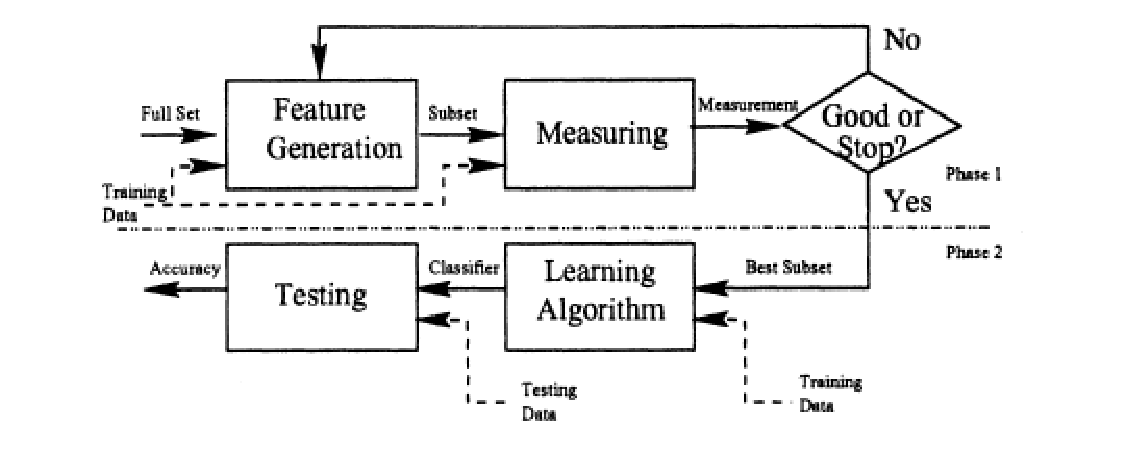
\includegraphics[keepaspectratio=true,scale=1]{figuras/fig05.eps}
	\caption{Fluxograma do modelo de filtro (\textit{filter}). \cite{huan_1998}}
\end{figure}

O modelo é composto por duas fases, a primeira fase consiste em seleção de características utilizando as medidas descritas no capítulo anterior, a segunda fase consiste em utilizar o subconjunto gerado em um classificador. Nessa fase também é colocado os dados de treino no classificador para avaliar se o resultado foi satisfatório. Os algoritmos de filtro não dependem da avaliação do classificador, e sim das informações e medidas obtidas diretamente dos dados. \cite{huan_1998}

Pode-se generalizar o modelo de filtro de acordo com a imagem 6, onde para um dado conjunto \textit{D} de características, é escolhido um subconjunto \textit{S0} através de alguma das formas de busca. Cada conjunto gerado é avaliado e comparado com o seu anterior, sempre sendo escolhido aquele que tenha um melhor valor em seu critério de avaliação ($\gamma$). Esse processo será repetido até que um critério de parada ($\alpha$) seja alcançado ou que sejam testados todos os conjuntos possíveis. \cite{liu_2005}

\begin{figure}[h]
	\centering
	\label{fig06}
		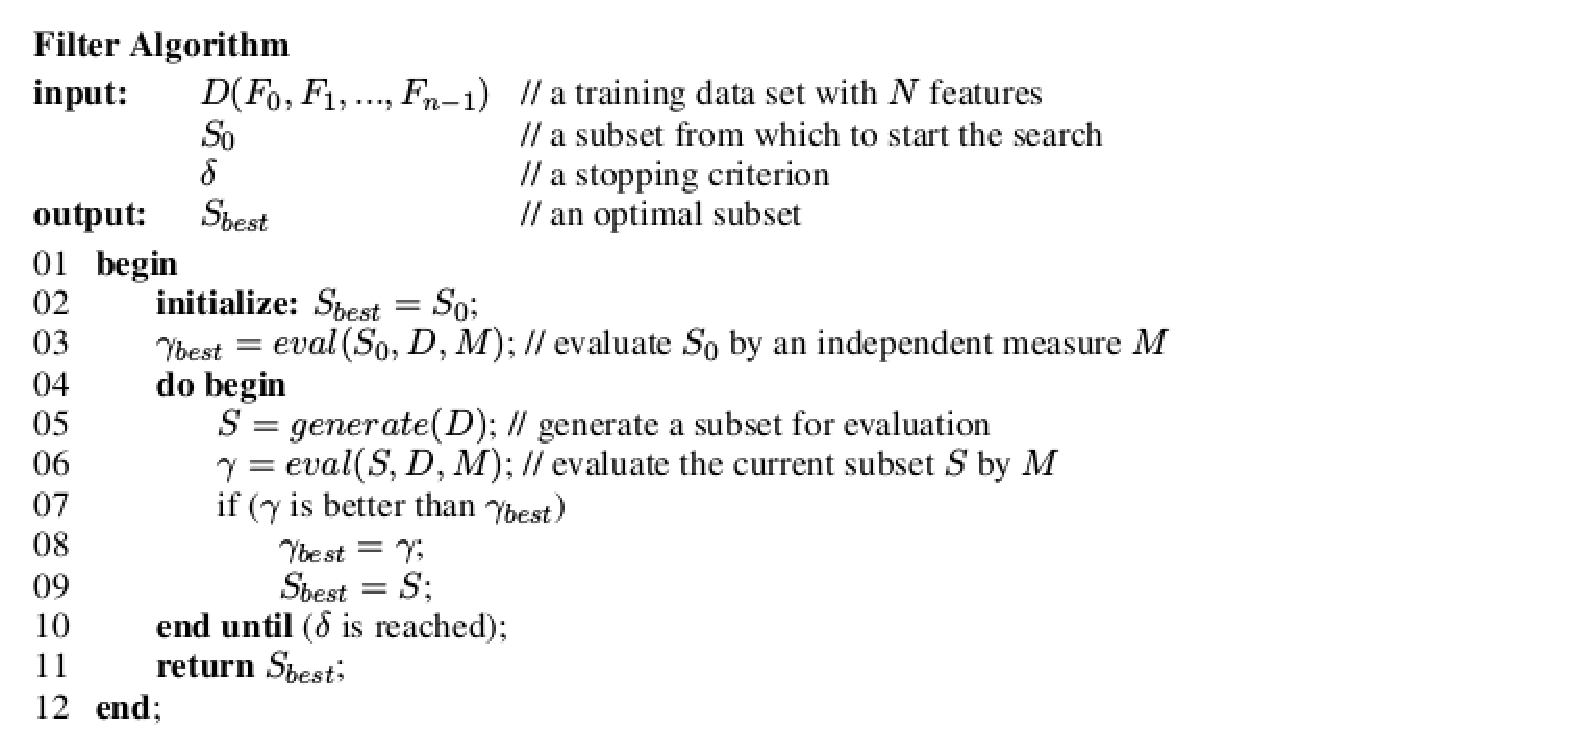
\includegraphics[keepaspectratio=true,scale=0.7]{figuras/fig07.eps}
	\caption{Generalização do algoritmo de filtro (\textit{filter}). \cite{liu_2005}}
\end{figure}

\subsection{Modelo de Envelopamento (\textit{wrapper})}

Os algoritmos que se baseiam no modelo de envelopamento necessitam de um algoritmo de \textit{machine learning} pré determinado para que seja possível utiliza-lo. Isso se deve ao fato de que o modelo usa o próprio classificador para avaliar o quão bom é o subconjunto de dados gerado. A imagem 7 ilustra como funciona um algoritmo de envelopamento.

\begin{figure}[h]
	\centering
	\label{fig07}
		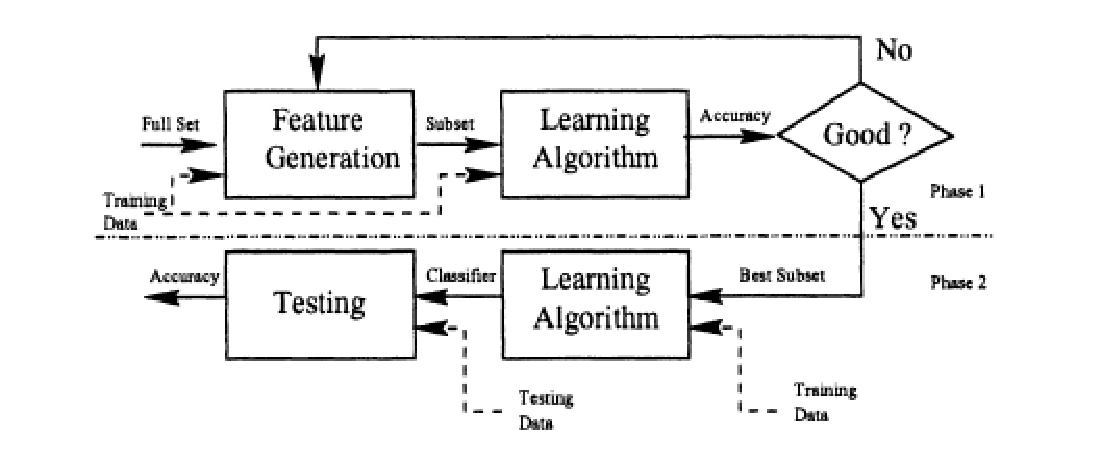
\includegraphics[keepaspectratio=true,scale=1]{figuras/fig06.eps}
	\caption{Fluxograma do modelo de envelopamento (\textit{wrapper}). \cite{huan_1998}}
\end{figure}

O modelo é composto por duas fases, a primeira fase consiste em escolher um subconjunto utilizando um classificador para poder avaliar o quão bom é esse modelo. Já a segunda fase é igual a do modelo de filtro, onde o subconjunto é utilizado no classificador e então são inseridos os dados de treino para verificar se o resultado foi satisfatório.

Pode-se generalizar o modelo de envelopamento de acordo com a imagem 8, onde para um dado conjunto \textit{D} de características, é escolhido um subconjunto \textit{S0} através de alguma das formas de busca. Cada conjunto gerado é avaliado e comparado com o seu anterior utilizando um algoritmo de \textit{machine learning}, sempre sendo escolhido aquele que tenha um melhor valor em seu critério de avaliação ($\gamma$). Esse processo será repetido até que um critério de parada ($\alpha$) seja alcançado ou que sejam testados todos os conjuntos possíveis. \cite{liu_2005}


\begin{figure}[h]
	\centering
	\label{fig08}
		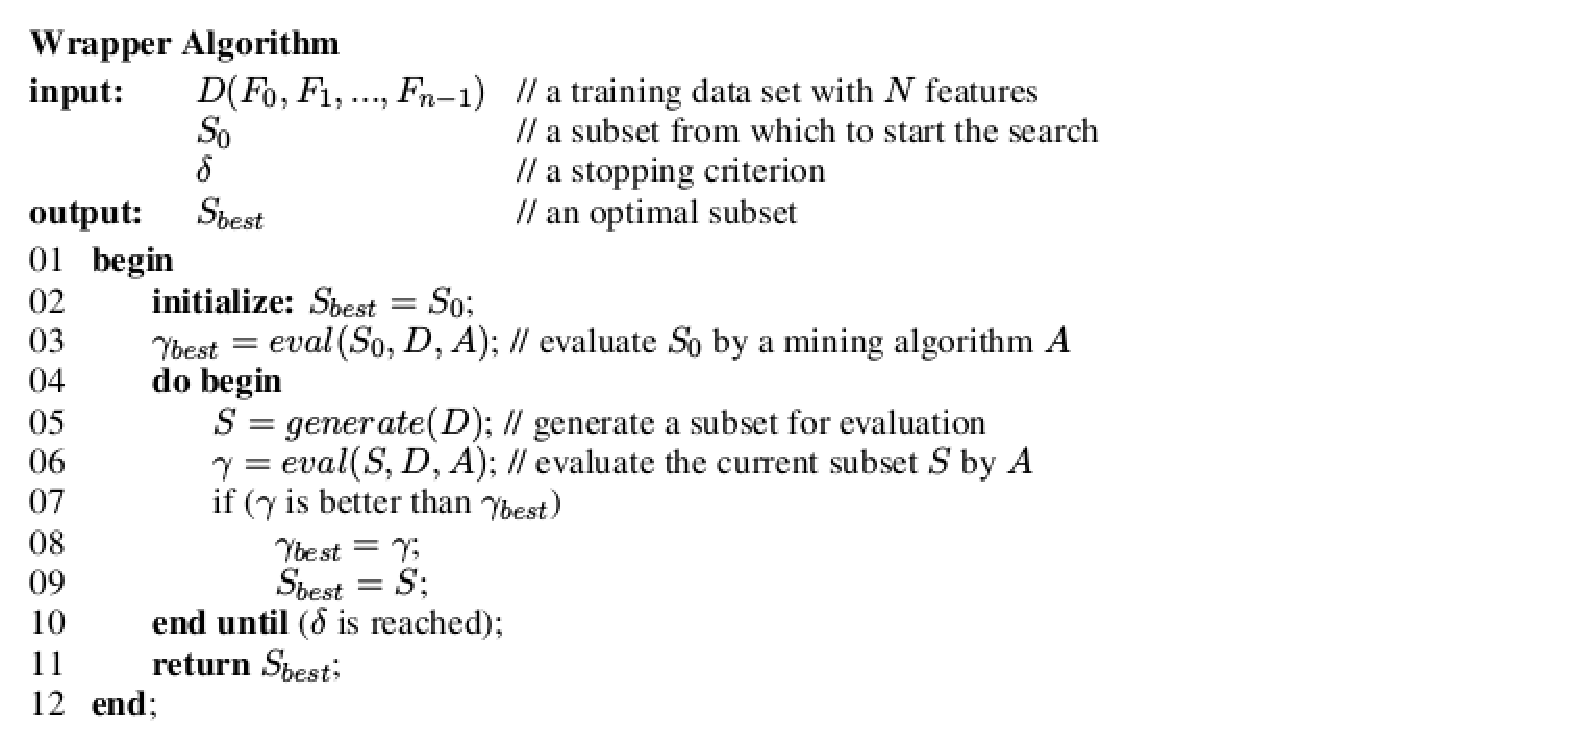
\includegraphics[keepaspectratio=true,scale=0.7]{figuras/fig08.eps}
	\caption{Generalização do algoritmo de envelopamento (\textit{wrapper}). \cite{liu_2005}}
\end{figure}

\subsection{Modelo Híbrido (\textit{hybrid})}

Os algoritmos que se baseiam no modelo híbrido são compostos por técnicas do modelo de filtro e de envelopamento. O modelo híbrido busca utilizar da melhor forma possível os dois modelos para poder alcançar um melhor subconjunto. Geralmente utiliza-se o modelo híbrido para problemas como muitos dados \cite{liu_2005}. Na figura 9 veremos como seu algorítimo funciona.

\begin{figure}[h]
	\centering
	\label{fig09}
		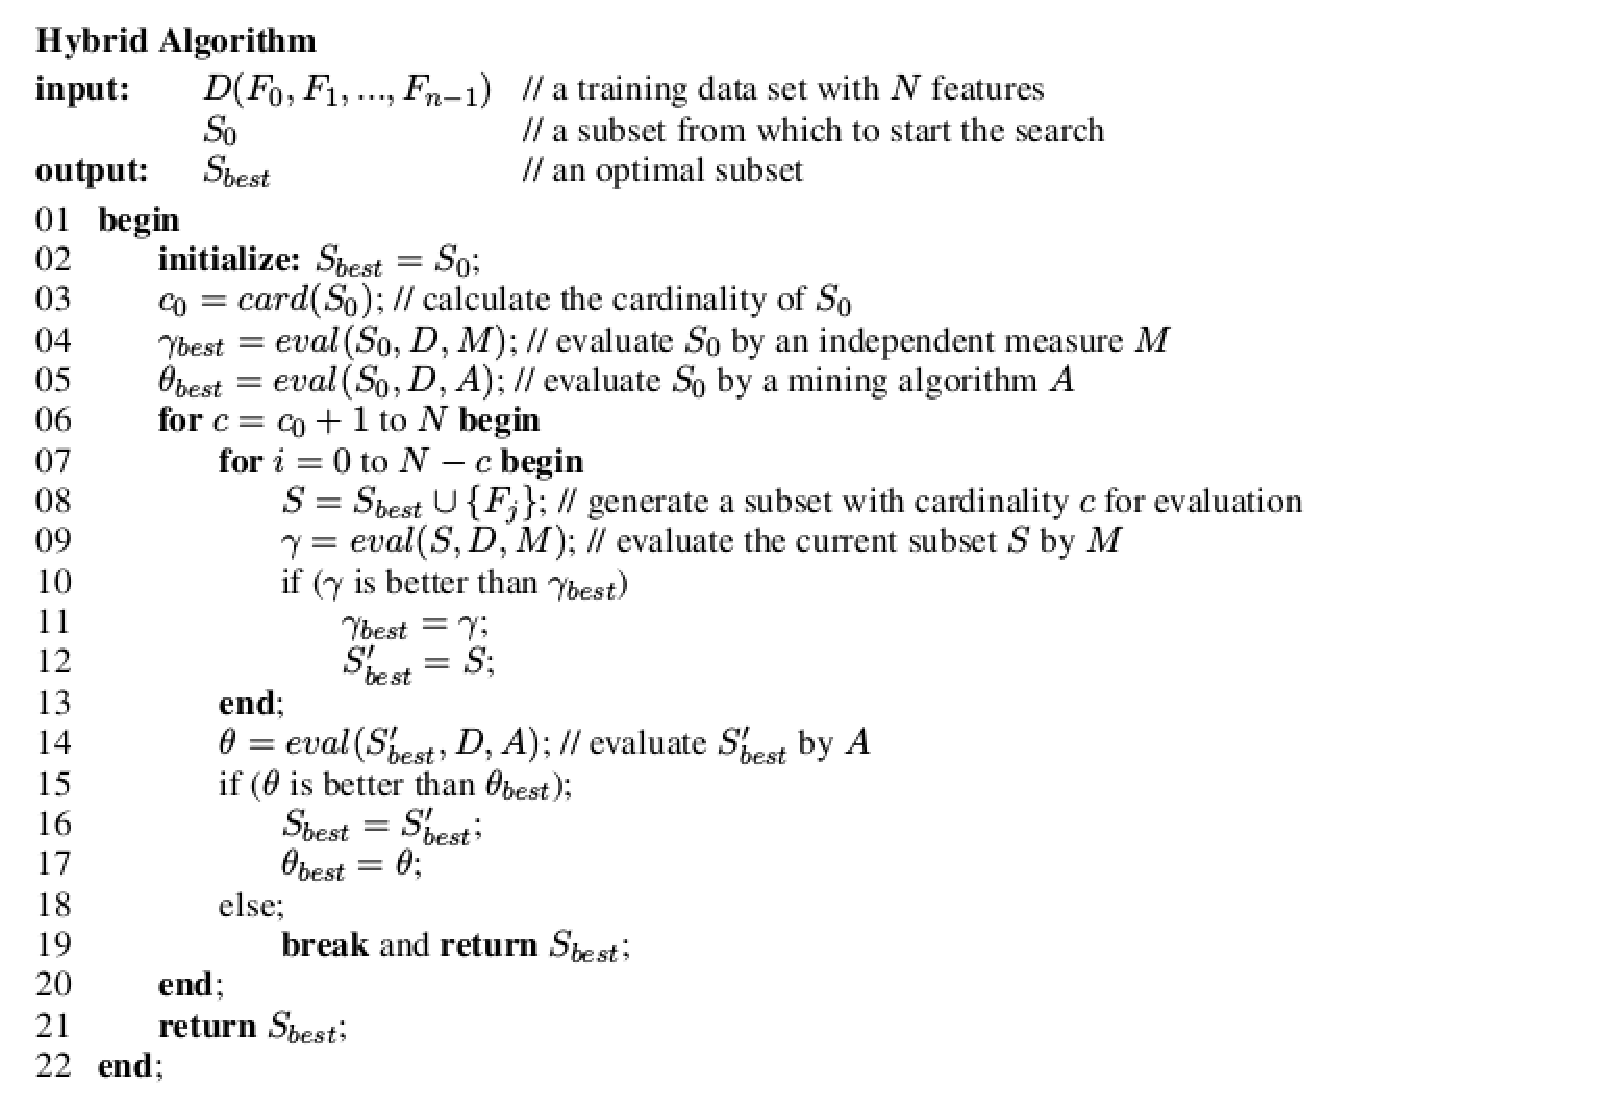
\includegraphics[keepaspectratio=true,scale=0.7]{figuras/fig09.eps}
	\caption{Generalização do algoritmo híbrido (\textit{hybrid}). \cite{liu_2005}}
\end{figure}

Para um dado conjunto \textit{D} de características, é escolhido um subconjunto \textit{S0} através de alguma das formas de busca, geralmente utiliza-se um conjunto vazio e é adicionado características a cada iteração. A cada iteração se adiciona uma característica e é comparada subconjunto a subconjunto dessa iteração utilizando medidas independentes ($\gamma$), ou seja, das características em si, que terá c + 1 características, até que seja possível encontrar o melhor subconjunto. Repete-se o processo até que se ache o melhor subconjunto de cada uma das iterações, e então esses subconjunto serão então comparados utilizando algum classificador ($\theta$), para que seja obtido o melhor subconjunto possível. \cite{liu_2005}

\section{Algoritmos Escolhidos}

\subsection{\textit{Relief}}

O algoritimo \textit{Relief} utiliza métodos estatísticos para selecionar as características relevantes, é um método que se baseia nos pesos atribuídos às caracterísicas \cite{dash_1997}. O algorítmo realiza a busca de maneira sequêncial e utiliza medidas de distância para poder realizar a avaliação entre as características. Primeiramente o algorítmo inicializa os pesos (\textit{W}) com 0, e escolhe um valor de limite ($\phi$), então para uma característica \textit{n} ele calcula os valores de \textit{Near Hit} e \textit{Near Miss}, ambos calculados através da distância euclidiana. \textit{Near Hit} é a menor distância entre instancias de mesma classe, já o \textit{Near Miss} é o menor valor entre instancias de classes diferentes. Depois de percorrer todas as características ele retorna aquelas que têm o valor do peso maior do que o limite estabelecido. O algoritmo funciona apenas para classes binárias. \cite{dash_1997}